\section{Empirical Validation} \label{sec:EmpiricalValidation}

This section provides an empirical validation of the Hypergeometric Volatility Model by comparing simulated implied volatility surfaces with observed market data. The analysis is based on S\&P~500 option data from the OptionMetrics database (accessed via WRDS) for March 2023.

A mean implied volatility surface is constructed on a fixed moneyness-maturity grid using linear interpolation to ensure comparability with the simulated surfaces. The evaluation proceeds in two steps. First, the simulation quality criteria from Section~\ref{subsec:SimulationQualityCriteria} are tested on the empirical surface. Second, the model is calibrated by identifying the parameter configuration that yields the closest fit to the market surface, measured by the Mean Squared Error (MSE).


\subsection{Empirical Volatility Surface} \label{subsec:EmpiricalVolatilitySurface}

\subsubsection*{Data Collection and Preparation}
S\&P~500 option data for March 2023 were obtained from the OptionMetrics database via WRDS. The dataset includes implied volatilities, strike prices, and expiration dates for listed equity index options.

Data cleaning was performed to remove extreme or invalid entries. Excluded were:
\begin{itemize}
    \item Implied volatilities above 100\%,
    \item Maturities longer than three years,
    \item Extremely deep in- or out-of-the-money options.
\end{itemize}
After cleaning, the dataset contained approximately 373{,}000 observations from March 1 to March 31, 2023. Maturities range from 1 day to 3 years, and strikes cover a wide range of moneyness values from $K/S = 0.3$ to $K/S = 3.1$. This provides a broad cross-section of the implied volatility surface across both short and long maturities.

Strike prices were converted to moneyness using the ratio $K/S$, and maturities were expressed in years. The data were binned onto a discrete moneyness-maturity grid, averaged within bins, and interpolated linearly. The resulting surface was evaluated on the same grid used in Section~\ref{sec:SimulationResultsAnalysis}, consisting of 17 moneyness levels
\begin{equation*}
    \{0.5,\, 0.7,\, 0.8,\, 0.9,\, 0.95,\, 0.975,\, 0.99,\, 0.995,\, 1,\, 1.005,\, 1.01,\, 1.025,\, 1.05,\, 1.1,\, 1.2,\, 1.4,\, 2\}
\end{equation*}
and 15 maturities (in trading days)
\begin{equation*}
    \{1,\, 2,\, 3,\, 5,\, 10,\, 15,\, 21,\, 42,\, 63,\, 84,\, 126,\, 252,\, 378,\, 504,\, 756\},
\end{equation*}
assuming 252 trading days per year. This grid yields 255 evaluation points at which empirical and simulated implied volatilities are compared directly, so that no additional interpolation is required during calibration.

\subsubsection*{Evaluation of Quality Criteria}
The empirical surface satisfies all four simulation quality criteria that can be evaluated based on implied volatilities. The put-call parity criterion cannot be tested, since OptionMetrics provides implied volatilities but not raw option prices.

Figure~\ref{fig:MarketSurface} and the associated diagnostics (volatility smiles, ATM skew, and log-log ATM skew term structure) confirm that the empirical surface exhibits the key stylized facts observed in financial markets: convex volatility smiles, a negative at-the-money skew, an increasing skew term structure, and approximate power-law decay. The regression on the log-log plot of the ATM skew against maturity achieves an $R^2$ value of 95.5\%, with an estimated decay exponent of $\gamma = 0.291$. Following \citet{Fukasawa2011}, this corresponds to an implied roughness parameter of $H = \tfrac{1}{2} - \gamma = 0.209$. These findings demonstrate that the empirical S\&P~500 surface is consistent with the quality criteria introduced in Section~\ref{subsec:SimulationQualityCriteria}, and thus provide a suitable benchmark for the calibration of the Hypergeometric Volatility Model.

\begin{figure}[H]
    \centering
    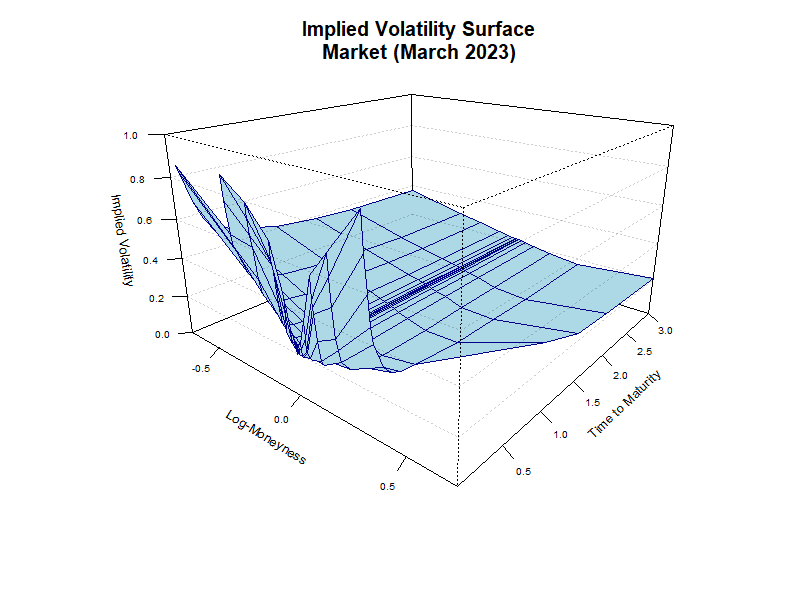
\includegraphics[width=0.45\textwidth]{figures/6.1 Market Surface/market_iv_surface.png}
    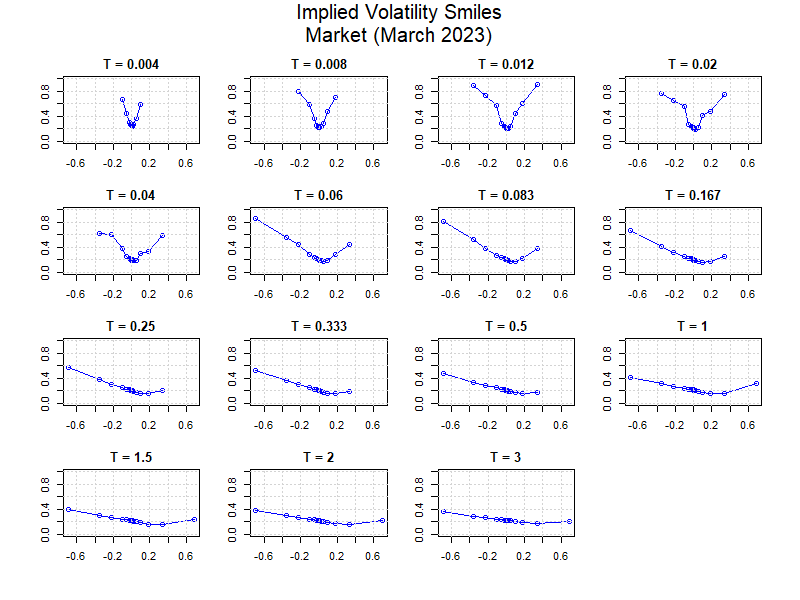
\includegraphics[width=0.45\textwidth]{figures/6.1 Market Surface/market_iv_smiles.png}
    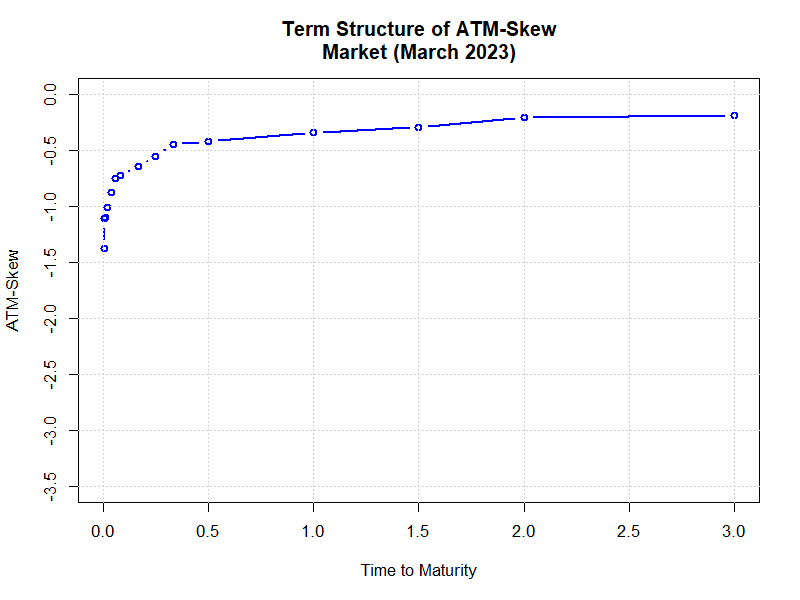
\includegraphics[width=0.45\textwidth]{figures/6.1 Market Surface/market_atm_skew.png}
    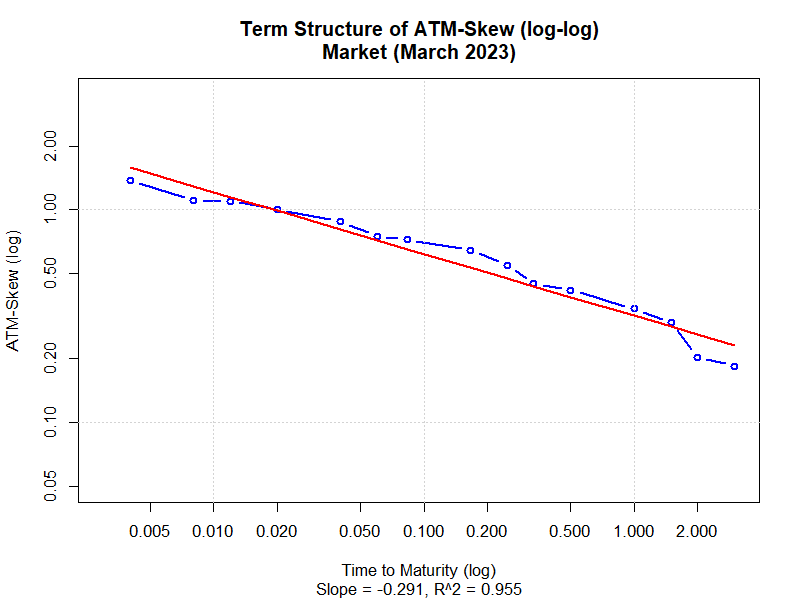
\includegraphics[width=0.45\textwidth]{figures/6.1 Market Surface/market_atm_skew_log.png}
    \caption{Empirical implied volatility surface, volatility smiles, ATM skew, and log-log skew term structure (S\&P~500; March 2023).}
    \label{fig:MarketSurface}
\end{figure}


\subsection{Calibration to Market Data}

\subsubsection*{Calibration Methodology}
The calibration was performed using a grid search approach. All 18{,}225 parameter configurations from the simulation study in Section~\ref{subsec:SuccessRateAnalysis} were evaluated through comparison of their simulated volatility surfaces with the empirical market surface from Section~\ref{subsec:EmpiricalVolatilitySurface}. For each scenario, the goodness of fit was assessed by the Mean Squared Error (MSE) computed over the predefined strikes-maturities grid:
\begin{equation}
    \text{MSE} = \frac{1}{N} \sum_{i=1}^{N} \left( \sigma_{\text{model}}^{(i)} - \sigma_{\text{market}}^{(i)} \right)^2,    
\end{equation}
where $\sigma_{\text{model}}^{(i)}$ and $\sigma_{\text{market}}^{(i)}$ denote the model-implied and market-implied volatilities at grid point $i$, and $N$ is the total number of grid points with valid data. The parameter set yielding the lowest MSE was identified as the best fit to the market surface.


\subsubsection*{Best Fit Parameter Set}
The configuration minimizing the MSE is
\begin{equation*}
    \{ H = 0.05,\quad \gamma_2 = 0.20,\quad \rho = -0.7,\quad a = 1.0,\quad b = 0.20,\quad r = 0.02,\quad J = 20 \}.
\end{equation*}

\begin{figure}[H]
    \centering
    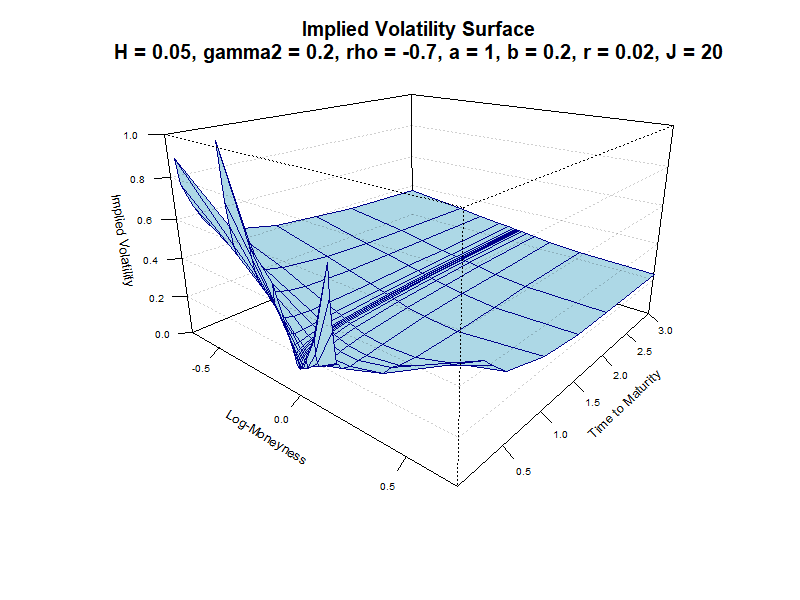
\includegraphics[width=0.45\textwidth]{figures/6.2 Best Fit Surface/best_fit1_iv_surface.png}
    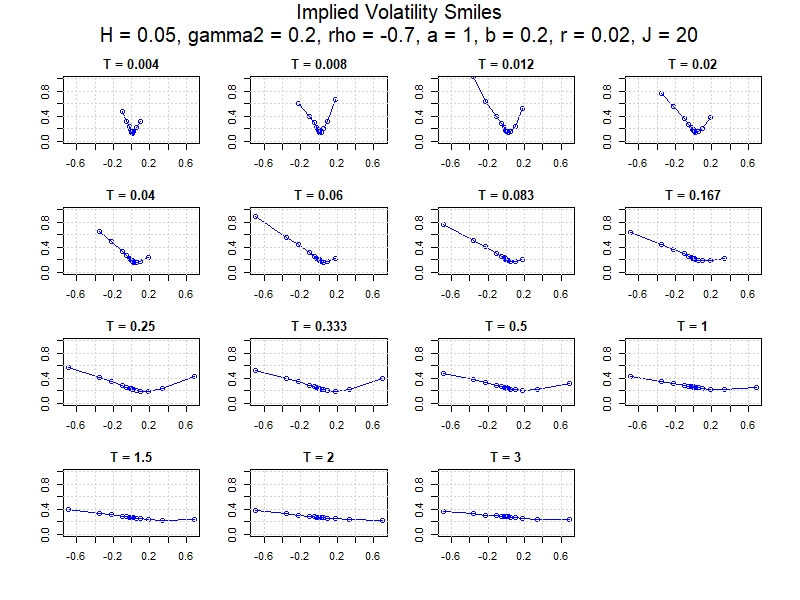
\includegraphics[width=0.45\textwidth]{figures/6.2 Best Fit Surface/best_fit1_iv_smiles.png}
    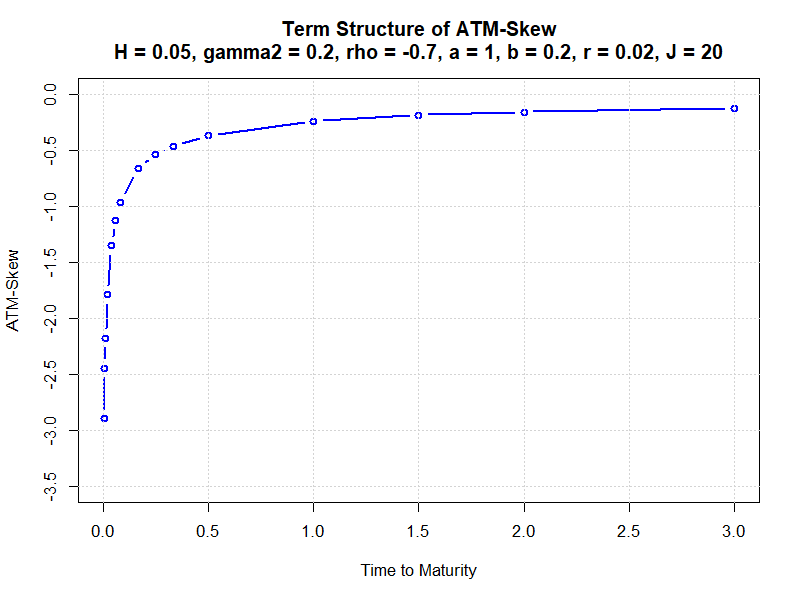
\includegraphics[width=0.45\textwidth]{figures/6.2 Best Fit Surface/best_fit1_atm_skew.png}
    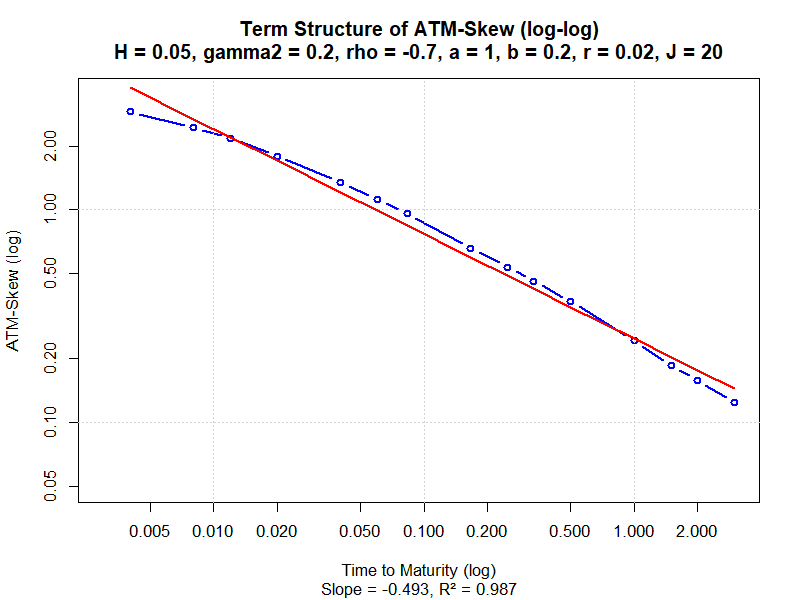
\includegraphics[width=0.45\textwidth]{figures/6.2 Best Fit Surface/best_fit1_atm_skew_log.png}
    \caption{Calibrated implied volatility surface, smile slices, ATM skew, and log-log skew term structure.}
    \label{fig:BestFitSurface}
\end{figure}

The calibrated surface in Figure~\ref{fig:BestFitSurface} reproduces the key characteristics of the S\&P~500 volatility surface. The overall shape of the volatility smiles, the negative and increasing ATM skew, and the approximate power-law decay are all matched with high accuracy. The strongest agreement is observed in the short-maturity and near-the-money region, where option prices are most liquid and reliable.

These results confirm that the Hypergeometric Volatility Model is capable of replicating essential stylized features of market volatility surfaces, provided that parameter values remain within the favorable ranges identified in Section~\ref{subsec:SuccessRateAnalysis}.